\documentclass[a4paper]{article}
\usepackage[spanish]{babel}
\usepackage[utf8]{inputenc}
\usepackage{charter}   % tipografia
\usepackage{graphicx}

%%%%%%%LO AGREGUE%%%%%%%%%%
\usepackage{hyperref}
%%%%%%%%%%%%%%%%%%%%%%%%%%

%\usepackage{makeidx}
\usepackage{paralist} %itemize inline
\usepackage[ruled,vlined]{algorithm2e}
%\usepackage{float}
%\usepackage{amsmath, amsthm, amssymb}
%\usepackage{amsfonts}
%\usepackage{sectsty}
%\usepackage{charter}
%\usepackage{wrapfig}
%\usepackage{listings}
%\lstset{language=C}


\usepackage{color} % para snipets de codigo coloreados
\usepackage{fancybox}  % para el sbox de los snipets de codigo

\definecolor{litegrey}{gray}{0.94}

% \newenvironment{sidebar}{%
% 	\begin{Sbox}\begin{minipage}{.85\textwidth}}%
% 	{\end{minipage}\end{Sbox}%
% 		\begin{center}\setlength{\fboxsep}{6pt}%
% 		\shadowbox{\TheSbox}\end{center}}
% \newenvironment{warning}{%
% 	\begin{Sbox}\begin{minipage}{.85\textwidth}\sffamily\lite\small\RaggedRight}%
% 	{\end{minipage}\end{Sbox}%
% 		\begin{center}\setlength{\fboxsep}{6pt}%
% 		\colorbox{litegrey}{\TheSbox}\end{center}}

\newenvironment{codesnippet}{%
	\begin{Sbox}\begin{minipage}{\textwidth}\sffamily\small}%
	{\end{minipage}\end{Sbox}%
		\begin{center}%
		\vspace{-0.4cm}\colorbox{litegrey}{\TheSbox}\end{center}\vspace{0.3cm}}



\usepackage{fancyhdr}
\pagestyle{fancy}

%\renewcommand{\chaptermark}[1]{\markboth{#1}{}}
\renewcommand{\sectionmark}[1]{\markright{\thesection\ - #1}}

\fancyhf{}

\fancyhead[LO]{Sección \rightmark} % \thesection\ 
\fancyfoot[LO]{\small{Agustina Aldasoro, Francisco Noriega, Ezequiel Zimenspitz, Brian Zuker}}
\fancyfoot[RO]{\thepage}
\renewcommand{\headrulewidth}{0.5pt}
\renewcommand{\footrulewidth}{0.5pt}
\setlength{\hoffset}{-0.8in}
\setlength{\textwidth}{16cm}
%\setlength{\hoffset}{-1.1cm}
%\setlength{\textwidth}{16cm}
\setlength{\headsep}{0.5cm}
\setlength{\textheight}{25cm}
\setlength{\voffset}{-0.7in}
\setlength{\headwidth}{\textwidth}
\setlength{\headheight}{13.1pt}

\renewcommand{\baselinestretch}{1.1}  % line spacing


% \setcounter{secnumdepth}{2}
\usepackage{underscore}
\usepackage{caratula}
%\usepackage{url}
\usepackage{hyperref}

% ******************************************************** %
%              TEMPLATE DE INFORME ORGA2 v0.1              %
% ******************************************************** %
% ******************************************************** %
%                                                          %
% ALGUNOS PAQUETES REQUERIDOS (EN UBUNTU):                 %
% ========================================
%                                                          %
% texlive-latex-base                                       %
% texlive-latex-recommended                                %
% texlive-fonts-recommended                                %
% texlive-latex-extra?                                     %
% texlive-lang-spanish (en ubuntu 13.10)                   %
% ******************************************************** %



\begin{document}


\thispagestyle{empty}
\materia{Algoritmos y Estructuras de Datos III}
\submateria{Primer Cuatrimestre de 2015}
\titulo{Trabajo Práctico I}
%\subtitulo{subtitulo del trabajo}
\integrante{Aldasoro Agustina}{86/13}{agusaldasoro@gmail.com}
\integrante{Noriega Francisco}{XXX/XX}{mail}
\integrante{Zimenspitz Ezequiel}{155/13}{ezeqzim@gmail.com}
\integrante{Zuker Brian}{XXX/XX}{mail}


\maketitle
\newpage

\thispagestyle{empty}
\vfill
\begin{abstract}
Habi\'endonos sido dado una serie de tres problem\'aticas a resolver, se plantean sus respectivas soluciones acorde a los requisitos pedidos. Se adjunta una descripci\'on de cada problema y su soluci\'on, conjunto a su an\'alisis de correctitud y de complejidad sumado a su experimentaci\'on. El lenguaje elegido para llevar a cabo el trabajo es C++.
\end{abstract}

\thispagestyle{empty}
\vspace{3cm}
\tableofcontents
\newpage


%\normalsize
\newpage

\section{Problema 1: ZombieLand}

\subsection{Descripci\'on de la problem\'atica}

Dado un mapa con n ciudades, en cada una de ellas se encuentra una determinada cantidad de Zombies y una determinada cantidad de soldados (ambas tambi\'en dadas). El objetivo del problema es exterminar a la invasi\'on zombie, para ello es necesario un enfrentamiento \textit{zombies vs soldados} por cada ciudad. Con el fin de que este enfrentamiento sea positivo, es decir se logre matar a todos los zombies de una ciudad, es necesario que la cantidad de zombies sea, a lo sumo, diez veces m\'as grande que la cantidad de soldados.

Como los soldados se encuentran atrincherados, se puede optar entre llevar a cabo un enfrentamiento o no (ya que no se desea provocar un ataque donde ya se sabe que se va a perder). Los soldados acuartelados no pueden moverse de la ciudad en la que est\'an, pero s\'i se cuenta con una dotaci\'on de soldados extra que se la puede ubicar en cualquiera de las n ciudades acorde a lo deseado. La cantidad de soldados extra es ilimitada, mas los recursos para trasladarlos no lo son. El traslado de cada soldado extra a una ciudad tiene un costo espec\'ifico que var\'ia acorde a la ciudad elegida. Siempre que sea econ\'omicamente posible, se puede trasladar una cantidad de soldados indistinta por ciudad.

Debido a que los recursos econ\'omicos son finitos, no siempre va a ser posible salvar a las n ciudades. Lo que se desea en este problema es maximizar la cantidad de ciudades salvadas, respetando el presupuesto. Es decir, se deben dar las cantidades de soldados necesarias para cada ciudad de modo que la cantidad de ciudades salvadas sea la \'optima.  El algoritmo debe tener una complejidad temporal de $O(n.log(n))$, siendo $n$ la cantidad de ciudades del pa\'is.\\

\textcolor{blue}{Aca se podr\'ia poner unos dibujitos de soluciones \'optimas como para que quede m\'as lindo}



\subsection{Resoluci\'on propuesta y justificaci\'on}

Para la resoluci\'on del problema decidimos utilizar un algoritmo goloso, el mismo tomar\'a una decisi\'on \'optima para cada instante, sin revisar si ser\'a la mejor a nivel global.

El algoritmo simplemente calcula cu\'anto ser\'ia el costo de salvar a cada ciudad:
	\begin{codesnippet}
	\begin{verbatim}
		soldados_necesarios = redondeo_hacia_arriba((zombies - (soldados x 10)) /10)
		costo_total = costo_unitario * soldados_necesarios
	\end{verbatim}
	\end{codesnippet}

Ordena las ciudades de menor a mayor en base al costo de salvarla, y luego, secuencialmente, env\'ia los ej\'ercitos requeridos, respetando este orden, hasta que el pa\'is se queda sin presupuesto.

El algortimo resuelve el problema salvando la mayor cantidad de ciudades posibles porque
\textcolor{blue}{INSERT FORMAL DEMO}

\subsection{An\'alisis de la complejidad}
La complejidad de nuestra soluci\'on es $O(n.log(n))$, siendo $n$ la cantidad de ciudades del pa\'is.\\

El c\'odigo presenta un primer ciclo for que calcula el costo de salvar a cada ciudad y las agrega mediante push_back() a un vector. El ciclo recorre linealmente todas las ciudades y tiene complejidad $O(n)$. La funci\'on \href{http://www.cplusplus.com/reference/vector/vector/push_back/}{push_back()} tiene costo $O(1)$ amortizado, lo que implica que cuando no precisa redimensionar el vector cuesta esto, y cuando lo hace, toma tiempo lineal en la cantidad de elementos. Como insertamos durante todo el ciclo tomamos el costo amortizado y la complejidad nos da $O(n)$

Le sigue ordenar el arreglo con estos datos, para ello usamos \href{(http://www.cplusplus.com/reference/algorithm/sort_heap/?kw=sort_heap)}{heapsort} de la librer\'a de $C$ cuya complejidad es $O(n.log(n))$.

Finalmente se realiza otro ciclo for que salva las ciudades que pueda, mientras dure el presupuesto y deja en 0 soldados enviados a las ciudades que no pueden ser salvadas por optar por salvar a la mayor cantidad de ciudades posibles. Este ciclo recorre linealmente todas las ciudades y tiene complejidad $O(n)$.

\textcolor{blue}{La complejidad de como escribir la salida no me parece relevante... habr\'ia que preguntarlo}

Como cada paso de los mencionados son secuenciales, las complejidades se suman, obteniendo $O(n)$ + $O(n.log(n))$ + $O(n)$ que es igual a $O(n.log(n))$ por propiedades de $O$.

%	\begin{codesnippet}
%	\begin{verbatim}
%
%		struct Pepe {
%
%			...
%
%		};
%
%	\end{verbatim}
%	\end{codesnippet}

\newpage

\subsection{C\'odigo fuente}

\begin{algorithm}[h!]
\NoCaptionOfAlgo
\caption{Ejemplo de Algoritmo}
\For{cada fila de la imagen}{
	\For{cada columna de la imagen}{
		\eIf{es una fila de rojos y verdes}{
			\eIf{es un p\'ixel rojo}{
				canal verde $\leftarrow$ canal verde del p\'ixel de arriba\\
				canal azul $\leftarrow$ canal azul del p\'ixel de arriba a la izquierda			
			}{
				//Pixel Verde\\
				canal rojo $\leftarrow$ canal rojo del p\'ixel de la derecha\\
				canal azul $\leftarrow$ canal azul del p\'ixel de arriba			
			}
		}{
			//Fila de azules y verdes \\
			\eIf{es un p\'ixel verde}{
				canal rojo $\leftarrow$ canal rojo del p\'ixel de arriba\\
				canal azul $\leftarrow$ canal azul del p\'ixel de la izquierda			
			}{
				//P\'ixel Azul\\
				canal rojo $\leftarrow$ canal rojo del p\'ixel de abajo a la derecha\\
				canal verde $\leftarrow$ canal verde del p\'ixel de la derecha			
			}
		}
	}
}
\end{algorithm}


\subsection{Experimentaci\'on}

\newpage

\section{Problema 2: Alta Frecuencia}
\subsection{Descripci\'on de la problem\'atica}

Se quiere transmitir informaci\'on secuencialmente mediante un enlace el mayor tiempo posible. Los enlaces tienen asociadas distintas frecuencias, con un costo por minuto y un intervalo de tiempo (sin cortes) en el cual funcionan. Se utilizan durante minutos enteros, y es posible cambiar de una frecuencia a otra instant\'anemente (del minuto 1 al 4 uso la frecuencia A y del 4 al 6 la B. Los datos del precio y e intervalo de tiempo de cada frecuencia son dados. Se desea optimizar este problema para transmitir todo el tiempo que tenga al menos una frecuencia abierta, pero gastando la menor cantidad de dinero. Se debe contar con una complejidad de $O(n.log(n))$.

\textcolor{blue}{Aca poner ejemplitos de cual es la solucion optima cuando hay varias senales y cuando tenes que camibar de senial porque se prendio una mas barata.}

\subsection{Resoluci\'on propuesta y justificaci\'on}

%Analizar minuto a minuto cual es el mas barato es fuerza bruta?? -> Esto es cant de minutos x n

%Fijarse cual es el primer minuto que se tiene senial y cual es el ultimo
%Pagar siempre el mas barato en toda la frecuencia que haya
%revisar los baches que hayan quedado entre el minimo y el maximo, contratando desde el mas barato al mas caro
% ESTO ES N**2

%divide & conquer
%Fijarse cual es el primer minuto que se tiene senial y cual es el ultimo
%Ir dividiendo estos tiempos hasta casos base... 
%para mi el caso base es donde todas las frecuencias que hay pertenecen a ese intervalo fijo, porque sino no llegarias nunca a un caso base. Y cuando tenes un intervalo donde todas las frecuencias son parejas, ahi elegis la mas barata
%o el caso base es cuando llegas a intervalos de 1 minuto??? cosa que ahi tenes que determinar uno solo?

\subsection{An\'alisis de la complejidad}
\subsection{C\'odigo fuente}
\subsection{Experimentaci\'on}



\newpage

\section{Problema 3: El se\~nor de los caballos}
\subsection{Descripci\'on de la problem\'atica}

En este problema, se presenta un tablero de ajedrez de tama\~no $nxn$, el cual cuenta con alguna cantidad de caballos ubicados en una posici\'on aleatoria del tablero. Lo que se quiere lograr es \emph{cubrir} todo el tablero. Un casillero se considera cubierto si hay un caballo en \'el o bien, si es una posici\'on en la cual alg\'un caballo existente puede moverse con un s\'olo movimiento. Para lograr este cometido, puede ser necesario agregar nuevas fichas \emph{caballo} al tablero. No existe un l\'imite en la cantidad de caballos para agregar, pero lo que se busca es dar una soluci\'on con la m\'inima cantidad de caballos posibles.\\


En la figura \ref{caballito} se pueden ver todas las casillas que est\'an cubiertas por un s\'olo caballo.


 \begin{figure}[h!]
   \begin{center}
 	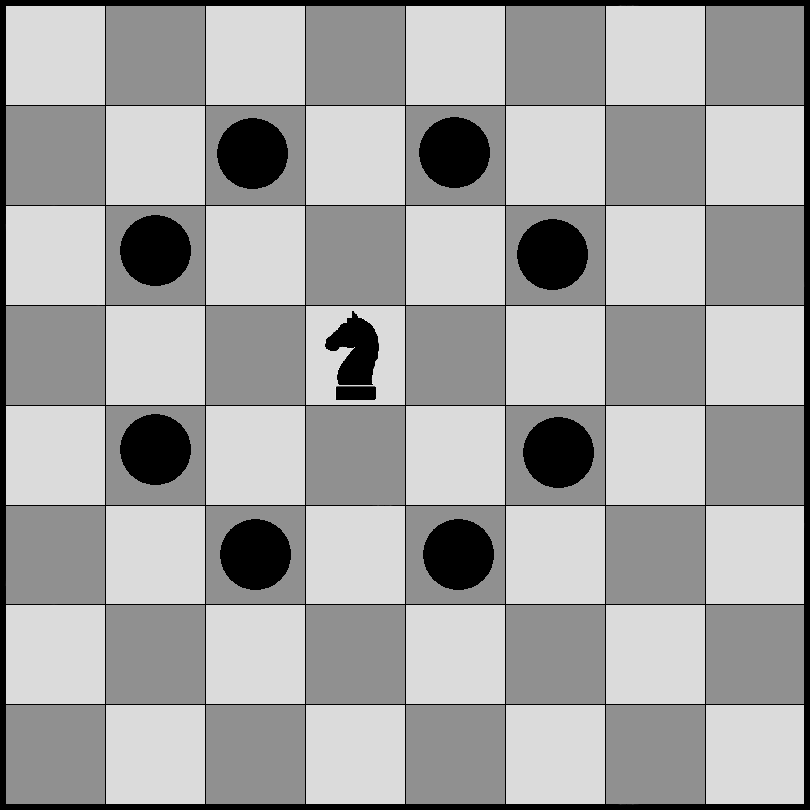
\includegraphics[scale=0.3]{imagenes/ej3/caballito.png}
 	\caption{Casillas que \emph{cubre} un caballo}
 	\label{caballito}	
 %	\href{http://www.fide.com/component/handbook/?id=124\&view=article}{Fuente}
   \end{center}
 \end{figure}


A continuaci\'on se pueden apreciar dos soluciones al problema de cubrir el tablero.

 \begin{figure}[h!]
   \begin{center}
 	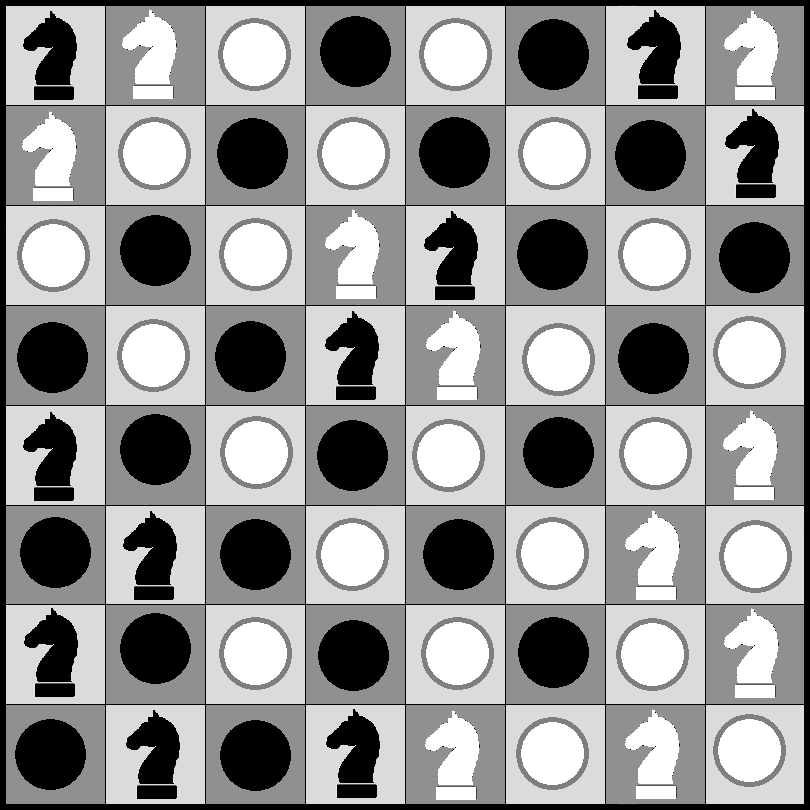
\includegraphics[scale=0.3]{imagenes/ej3/optimaCreo.png}
 	\caption{Soluci\'on 1}
% 	\label{optima_creo}	
   \end{center}
 \end{figure}
 
\newpage 
 
 
 \begin{figure}[h!]
   \begin{center}
 	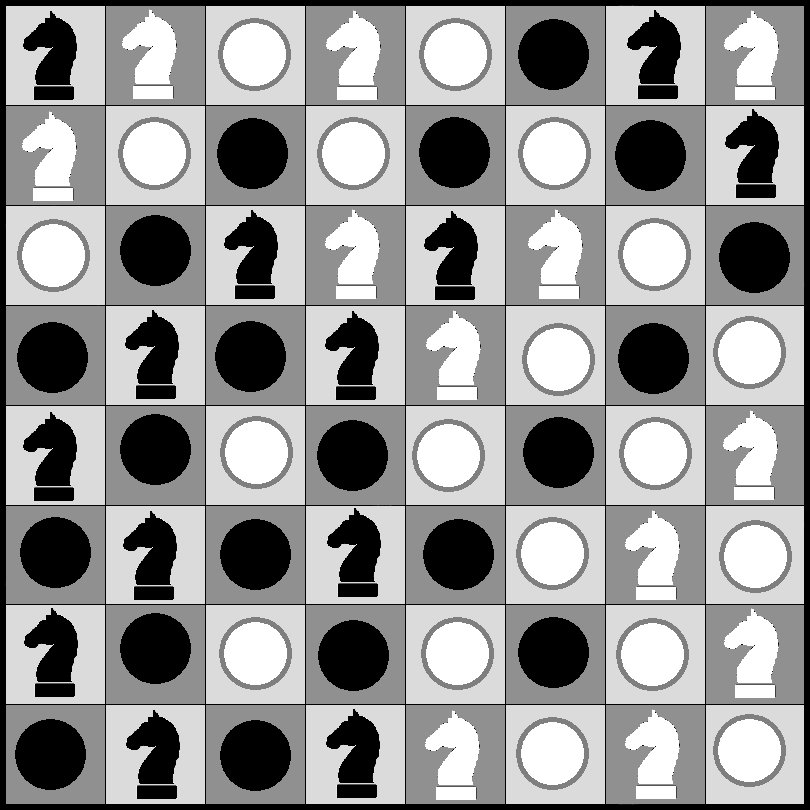
\includegraphics[scale=0.3]{imagenes/ej3/con5mas.png}
 	\caption{Soluci\'on 2}
 %	\label{con5mas}	
   \end{center}
 \end{figure}

En la soluci\'on 1 se necesitaron 20 caballos, en cambio en la dos 25; es decir 5 caballos m\'as. Por lo tanto podemos establecer que la soluci\'on 2 no es la \'optima y este caso no es lo que buscamos resolver. Por otro lado, la figura 1 \textcolor{red}{es \'optima? Despu\'es sabremos...}

\subsection{Resoluci\'on propuesta y justificaci\'on}

%re jodido esto amigooooo
%se ahcen todas las combinaciones y se va guardando la que tenga menor cantidad de caballos?

\subsection{An\'alisis de la complejidad}
\subsection{C\'odigo fuente}
\subsection{Experimentaci\'on}


% \section{Objetivos generales}

% El objetivo de este Trabajo Práctico es ...


% \section{Contexto}

% \begin{figure}
%   \begin{center}
% 	
\includegraphics[scale=0.66]{imagenes/logouba.jpg}
% 	\caption{Descripcion de la figura}
% 	\label{nombreparareferenciar}
%   \end{center}
% \end{figure}


% \paragraph{\textbf{Titulo del parrafo} } Bla bla bla bla.
% Esto se muestra en la figura~\ref{nombreparareferenciar}.




%Habra que insertar el enunciado???
% %\section{Enunciado y solucion} 
% %\input{enunciado}

% \section{Conclusiones y trabajo futuro}


\end{document}

